\documentclass[xcolor={dvipsnames},aspectratio=169,10pt]{beamer}
\usefonttheme{serif}

\makeatletter
  \def\beamer@calltheme#1#2#3{%
    \def\beamer@themelist{#2}
    \@for\beamer@themename:=\beamer@themelist\do
    {\usepackage[{#1}]{\beamer@themelocation/#3\beamer@themename}}}

  \def\usefolder#1{
    \def\beamer@themelocation{#1}
  }
  \def\beamer@themelocation{}
%%REF: https://tex.stackexchange.com/questions/275600/beamer-themes-on-custom-folder

\usefolder{../beamer_files}
\usetheme{mx}



\title{Finding a fETus with UltraSound (FETUS)}
\subtitle{Westminster STEAM Week {\bf \#WSW2022} }
\author{
  Thea Bautista, Goosie Leung and \\
  {\bf Miguel Xochicale}
}
\date{
15th March 2022
}
\institute{
	\faEnvelope \hspace{1mm}  miguel.xochicale@kcl.ac.uk \\
	\faGithubAlt \hspace{1mm}  @mxochicale
    \faTwitter \hspace{1mm}  @\_mxochicale
		}
\githubrepository{https://github.com/xfetus/pe}

\begin{document}

{
  \usebackgroundtemplate{\includegraphics[width=\paperwidth]{./../figures/background-for-titlepage/versions/drawing-v03.png}}
  \maketitle
}


\begin{frame}{Contents}
    \tableofcontents
\end{frame}

%%%%%%%%%%%%%%%%%%%%%%%%%%%%%%%%%%%%%%%%%%%%
\section{Who?, Why? Where?}


%%%%%%%%%%%%%%%%%%%%%%%%%%%%%%%%%%%%%%%%%%%%%
%\subsection{FETUS}

%%%%%%%%%%%%%%%%%%%%%%%%%%%%%%%%%%%%%%%%%%%%%%%%%%%%%%%%
{
%\paper{Lastname N. YEAR in journal of...}
\begin{frame}{Miguel Xochicale}
  %Who are we? / Where we come from? / Do we have hobbies?

  \begin{figure}
  \centering
  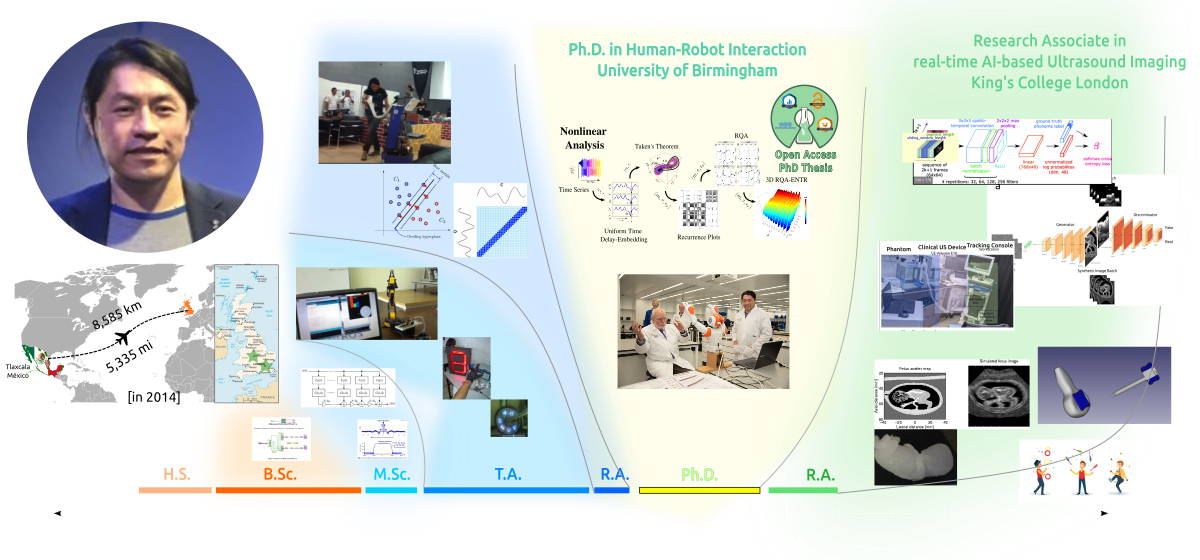
\includegraphics[width=1.0\textwidth]{./../figures/team/miguel-xochicale/versions/drawing-v05.png}
  \end{figure}

\end{frame}
}


%%%%%%%%%%%%%%%%%%%%%%%%%%%%%%%%%%%%%%%%%%%%%
%\subsection{FETUS}

%%%%%%%%%%%%%%%%%%%%%%%%%%%%%%%%%%%%%%%%%%%%%%%%%%%%%%%%
{
%\paper{Lastname N. YEAR in journal of...}
\begin{frame}{\faUsers Thea and Gooise}
    %Who are we? / Where we come from? / Do we have hobbies?

  \begin{figure}
  \centering
  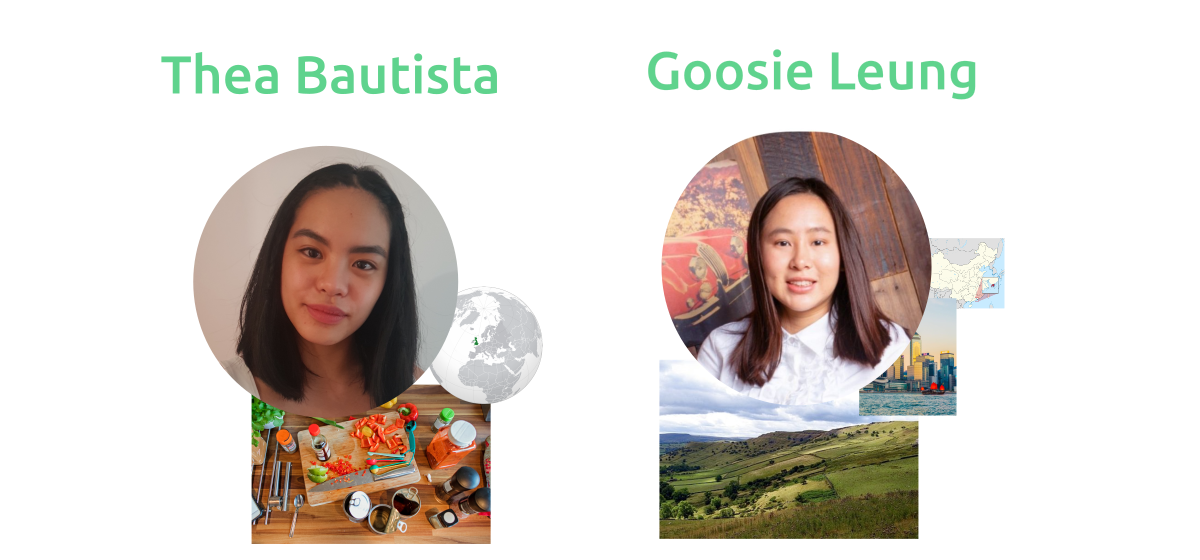
\includegraphics[width=1.0\textwidth]{./../figures/team/who-we-are/versions/drawing-v12.png}
  \end{figure}

\end{frame}
}



%%%%%%%%%%%%%%%%%%%%%%%%%%%%%%%%%%%%%%%%%%%%%
%\subsection{FETUS}

%%%%%%%%%%%%%%%%%%%%%%%%%%%%%%%%%%%%%%%%%%%%%%%%%%%%%%%%
{
%\paper{Lastname N. YEAR in journal of...}
\begin{frame}{Where we are based?}

  \begin{figure}
  \centering
  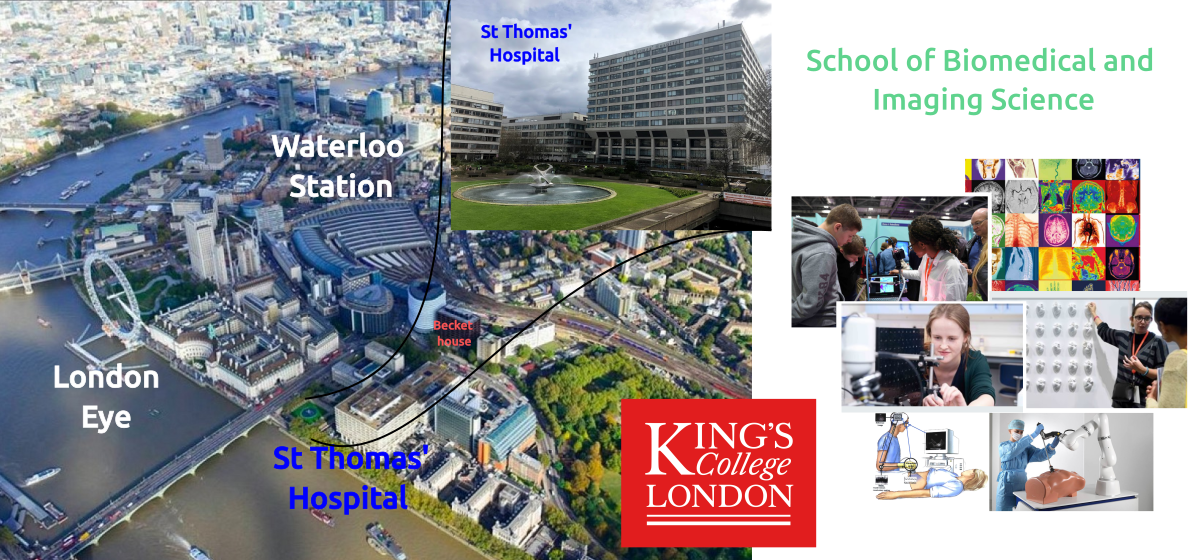
\includegraphics[width=1.0\textwidth]{./../figures/where-we-are-based/versions/drawing-v04.png}
  \end{figure}

\end{frame}
}



%%%%%%%%%%%%%%%%%%%%%%%%%%%%%%%%%%%%%%%%%%%%%
%\subsection{FETUS}

%%%%%%%%%%%%%%%%%%%%%%%%%%%%%%%%%%%%%%%%%%%%%%%%%%%%%%%%
{
\paper{\faExternalLinkSquare \hspace{1mm}  \url{https://www.kcl.ac.uk/bmeis}}
\begin{frame}{}

  \begin{figure}
  \centering
  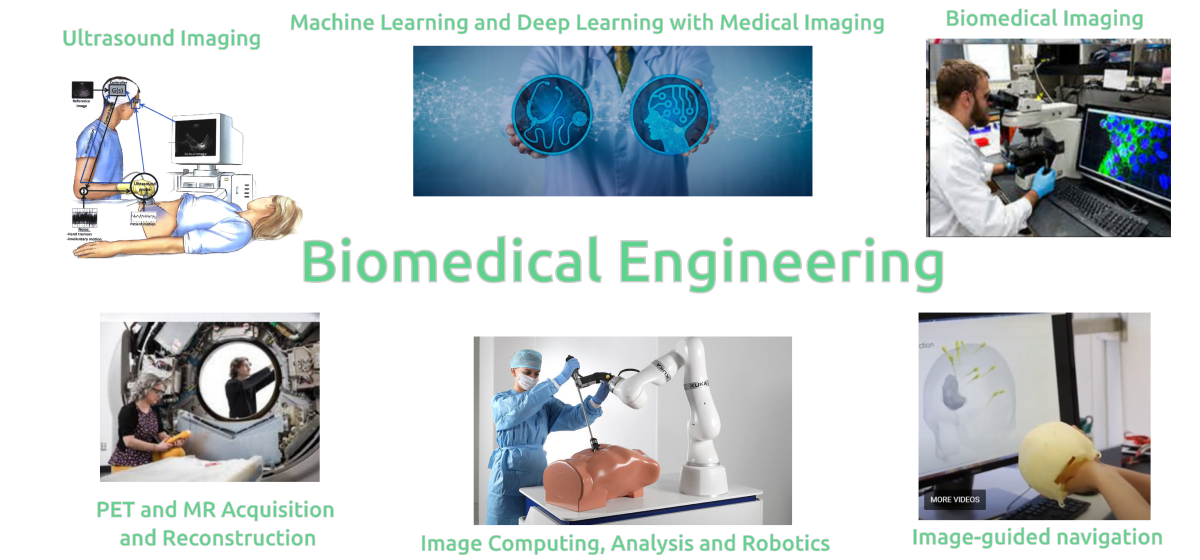
\includegraphics[width=1.0\textwidth]{./../figures/biomedical-engineer/versions/drawing-v04}
  \end{figure}

\end{frame}
}


%%%%%%%%%%%%%%%%%%%%%%%%%%%%%%%%%%%%%%%%%%%%%
%\subsection{FETUS}

%%%%%%%%%%%%%%%%%%%%%%%%%%%%%%%%%%%%%%%%%%%%%%%%%%%%%%%%
{
\paper{\faYoutubePlay \hspace{1mm}  \url{https://www.youtube.com/watch?v=iLZmT_fZqQo}}
\begin{frame}{Faculty of Life Sciences \& Medicine: video}

  \begin{figure}
  \centering
  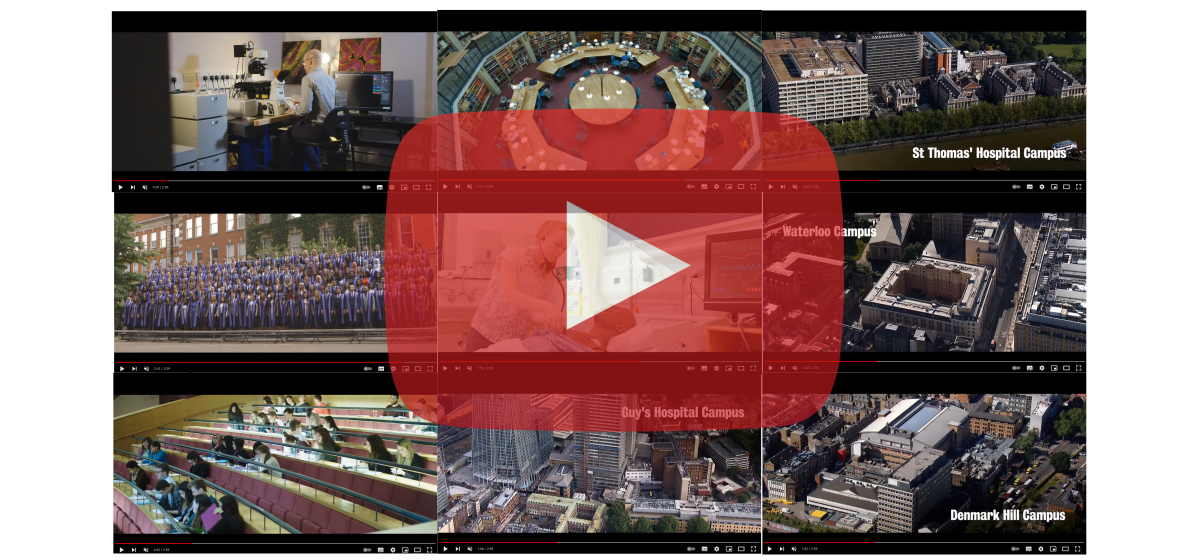
\includegraphics[width=1.0\textwidth]{./../figures/videos-life-science-and-medicine/versions/drawing-v00}
  \end{figure}

\end{frame}
}





%%%%%%%%%%%%%%%%%%%%%%%%%%%%%%%%%%%%%%%%%%%%%
%\subsection{FETUS}

%%%%%%%%%%%%%%%%%%%%%%%%%%%%%%%%%%%%%%%%%%%%%%%%%%%%%%%%
{
\paper{ \url{https://www.kcl.ac.uk/lsm/schools} }
\begin{frame}{}

  \begin{figure}
  \centering
  
\includegraphics[width=1.0\textwidth]{./../figures/schools-at-life-science-and-medicine/versions/drawing-v00}
  \end{figure}

\end{frame}
}


%%%%%%%%%%%%%%%%%%%%%%%%%%%%%%%%%%%%%%%%%%%%%
%\subsection{FETUS}

%%%%%%%%%%%%%%%%%%%%%%%%%%%%%%%%%%%%%%%%%%%%%%%%%%%%%%%%
{
\paper{\faWikipediaW \hspace{1mm} \url{https://en.wikipedia.org/wiki/Health_professional}}
\begin{frame}{}

  \begin{figure}
  \centering
  \includegraphics[width=1.0\textwidth]{./../figures/healthcare-professionals/versions/drawing-v03}
  \end{figure}

\end{frame}
}


%%%%%%%%%%%%%%%%%%%%%%%%%%%%%%%%%%%%%%%%%%%%%%%%%%%%%%%%%
%{
%%\paper{}
%\begin{frame}{}
%
%\BigSizeFont
%What does a Biomedical Engineer do?
%\end{frame}
%}
%





%%%%%%%%%%%%%%%%%%%%%%%%%%%%%%%%%%%%%%%%%%%%%%%%%%%%%%%%
{
%\paper{}
\begin{frame}{}

\BigSizeFont
Understanding Fetal Growth
%If you were a Sonographer for a day,
%what do you think would be the most challenging activities you would encounter?
\end{frame}
}




%%%%%%%%%%%%%%%%%%%%%%%%%%%%%%%%%%%%%%%%%%%%
\section{Guessing Fetal Growth}


%%%%%%%%%%%%%%%%%%%%%%%%%%%%%%%%%%%%%%%%%%%%%%%%%%%%%%%%
{
\paper{Growing Baby: 3D Print-ready Models;  \faWikipediaW \hspace{0.5mm} \url{https://en.wikipedia.org/wiki/Prenatal_development}  }
\begin{frame}{Understanding Fetal Growth}
      \begin{figure}
        \centering
        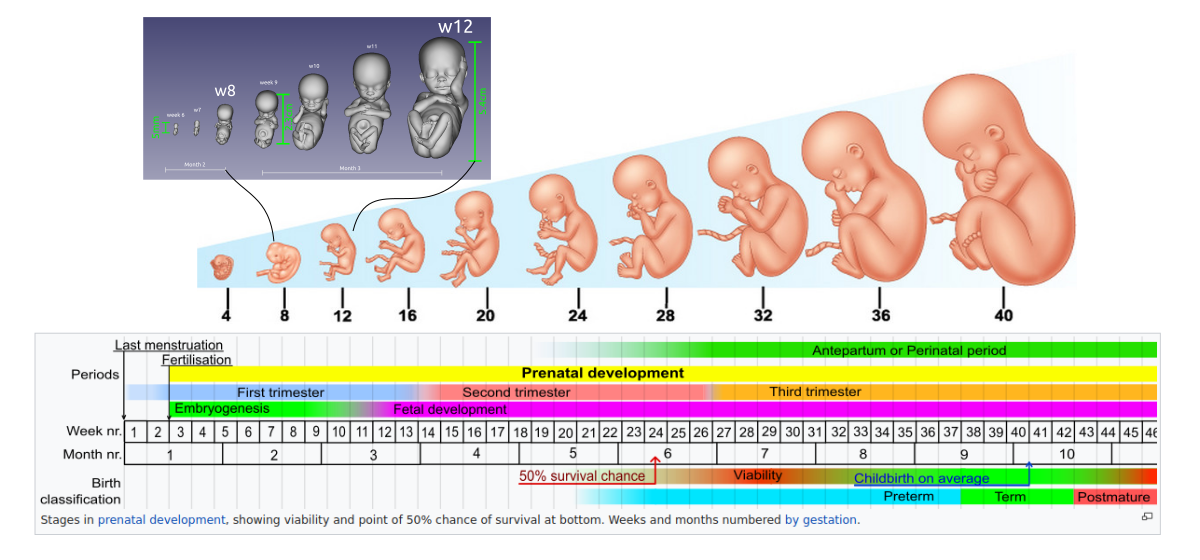
\includegraphics[width=1.0\textwidth]{./../figures/fetal-growth/versions/drawing-v02.png}
        %\caption{}
      \end{figure}
\end{frame}
}





%%%%%%%%%%%%%%%%%%%%%%%%%%%%%%%%%%%%%%%%%%%%%%%%%%%%%%%%
{
\paper{Growing Baby: 3D Print-ready Models}
\begin{frame}{[\faUsers ACTIVITY]: Drawing fetuses}
      \begin{figure}
        \centering
        \includegraphics[width=1.0\textwidth]{./../figures/fetal-growth-guess/versions/drawing-v03}
        %\caption{}
      \end{figure}
\end{frame}
}



%%%%%%%%%%%%%%%%%%%%%%%%%%%%%%%%%%%%%%%%%%%%%%%%%%%%%%%%
{
\paper{ de Bakker et al. 2016 in Science \url{http://3datlas.3dembryo.nl/}; \url{https://www.whattoexpect.com/pregnancy/}}
\begin{frame}{[\faUsers ACTIVITY]: Examples of fetuses at week-5 and week-6}
      \begin{figure}
        \centering
        \includegraphics[width=1.0\textwidth]{./../figures/fetal-size/versions/drawing-v01.png}
        %\caption{}
      \end{figure}
\end{frame}
}


%%%%%%%%%%%%%%%%%%%%%%%%%%%%%%%%%%%%%%%%%%%%%%%%%%%%%%%%
{
\paper{ de Bakker et al. 2016 in Science \url{http://3datlas.3dembryo.nl/}; \url{https://www.whattoexpect.com/pregnancy/}}
\begin{frame}{[\faUsers ACTIVITY]: Fetus at week-10}
      \begin{figure}
        \centering
        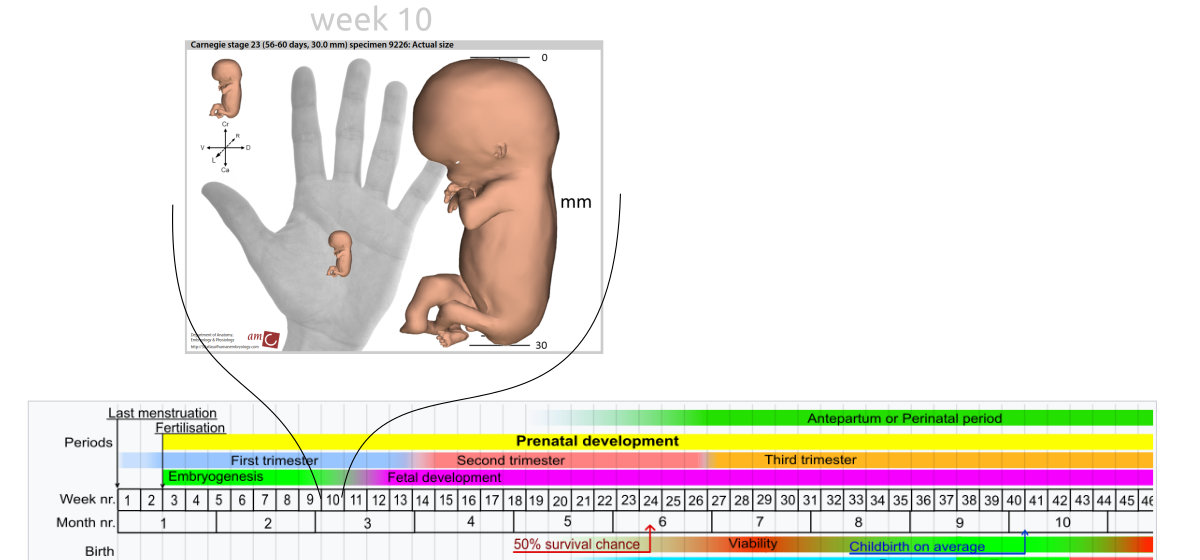
\includegraphics[width=1.0\textwidth]{./../figures/fetal-size/versions/drawing-v02.png}
        %\caption{}
      \end{figure}
\end{frame}
}



%%%%%%%%%%%%%%%%%%%%%%%%%%%%%%%%%%%%%%%%%%%%%%%%%%%%%%%%
{
%\paper{}
\begin{frame}{}

\BigSizeFont
\begin{center}
    Do you know what type of healthcare professional helps to monitor fetal development?
    %Do you know what is the role of a Sonographer?
\end{center}

\end{frame}
}


%%%%%%%%%%%%%%%%%%%%%%%%%%%%%%%%%%%%%%%%%%%%%%%%%%%%%%%%
{
\paper{Wright-Gilbertson M. 2014 in PhD thesis}
    \begin{frame}{Sonographer}
      \begin{figure}
        \centering
        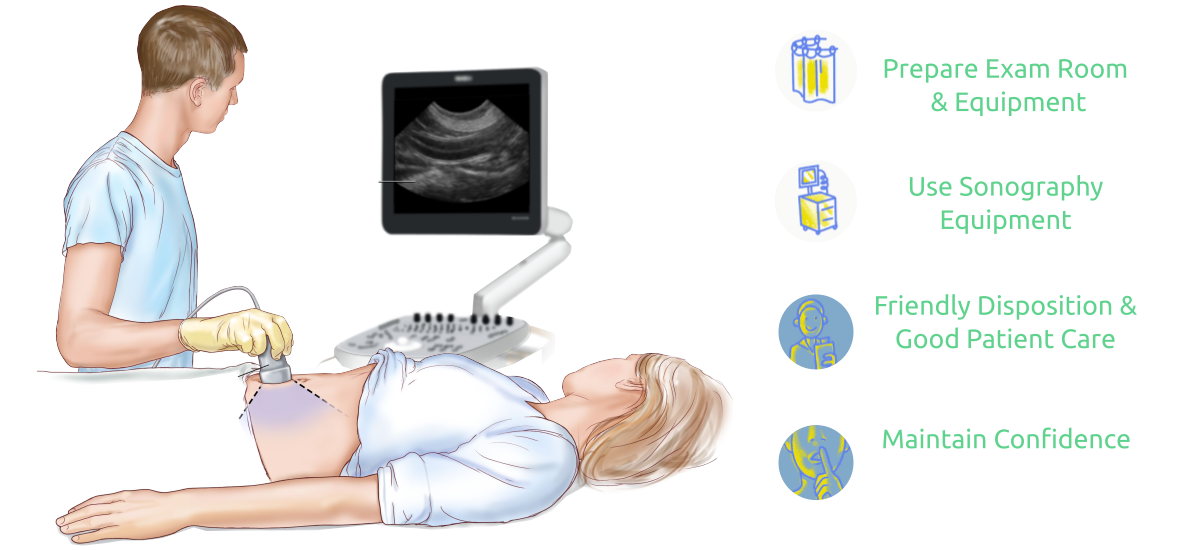
\includegraphics[width=1.0\textwidth]{./../figures/sonographer/versions/drawing-v02.png}
        %\caption{}
      \end{figure}
\end{frame}
}
%%%%%%%%%%%%%%%%%%%%%%%%%%%%%%%%%%%%%%%%%%%%
\section{Looking inside the human body}

%%%%%%%%%%%%%%%%%%%%%%%%%%%%%%%%%%%%%%%%%%%%%%%%%%%%%%%%
{
%\paper{}
\begin{frame}{}

\BigSizeFont
\begin{center}
    Do you know \\
    how clinitians can actually see fetal development?
\end{center}


\end{frame}
}


%%%%%%%%%%%%%%%%%%%%%%%%%%%%%%%%%%%%%%%%%%%%%%%%%%%%%%%%
{
\paper{\faWikipediaW \hspace{1mm} \url{https://en.wikipedia.org/wiki/Medical_imaging_in_pregnancy}}
\begin{frame}{Computational Tomography}
      \begin{figure}
        \centering
        \includegraphics[width=1.0\textwidth]{./../figures/medical-imaging-in-pregnancy/ct/versions/drawing-v01.png}
        %\caption{}
      \end{figure}
\end{frame}
}


%%%%%%%%%%%%%%%%%%%%%%%%%%%%%%%%%%%%%%%%%%%%%%%%%%%%%%%%
{
\paper{\faWikipediaW \hspace{1mm} \url{https://en.wikipedia.org/wiki/Medical_imaging_in_pregnancy}}
\begin{frame}{Magnetic Resonance Imaging}
      \begin{figure}
        \centering
        \includegraphics[width=1.0\textwidth]{./../figures/medical-imaging-in-pregnancy/mri/versions/drawing-v00.png}
        %\caption{}
      \end{figure}
\end{frame}
}


%%%%%%%%%%%%%%%%%%%%%%%%%%%%%%%%%%%%%%%%%%%%%%%%%%%%%%%%
{
\paper{\faWikipediaW \hspace{1mm} \url{https://en.wikipedia.org/wiki/Medical_imaging_in_pregnancy}}
\begin{frame}{Ultrasound}
      \begin{figure}
        \centering
        \includegraphics[width=1.0\textwidth]{./../figures/medical-imaging-in-pregnancy/us/versions/drawing-v02.png}
        %\caption{}
      \end{figure}
\end{frame}
}

%%%%%%%%%%%%%%%%%%%%%%%%%%%%%%%%%%%%%%%%%%%%%
%\subsection{FETUS}
%Medical imaging in pregnancy

%%%%%%%%%%%%%%%%%%%%%%%%%%%%%%%%%%%%%%%%%%%%%%%%%%%%%%%%
{
\paper{\faWikipediaW \hspace{1mm} \url{https://en.wikipedia.org/wiki/Medical_imaging_in_pregnancy}}
\begin{frame}{Medical Imaging in Pregnancy}
      \begin{figure}
        \centering
        \includegraphics[width=1.0\textwidth]{./../figures/medical-imaging-in-pregnancy/ct-mr-us/versions/drawing-v03.png}
        %\caption{}
      \end{figure}
\end{frame}
}



%{ % all template changes are local to this group.
%    \setbeamertemplate{navigation symbols}{}
%    \begin{frame}<article:0>[plain]
%        \begin{tikzpicture}[remember picture,overlay]
%            \node[at=(current page.center)] {
%                \includegraphics[keepaspectratio,
%                                 width=\paperwidth,
%                                 height=\paperheight]{./figures/medical-imaging-in-pregnancy/us/versions/drawing-v00.png}
%            };
%        \end{tikzpicture}
%     \end{frame}
%}


%%%%%%%%%%%%%%%%%%%%%%%%%%%%%%%%%%%%%%%%%%%%%
\section{Working in a Multidisciplinary team}


%%%%%%%%%%%%%%%%%%%%%%%%%%%%%%%%%%%%%%%%%%%%%%%%%%%%%%%%
{
%\paper{}
\begin{frame}{}

\BigSizeFont
\begin{center}
    Working in a Multidisciplinary team
\end{center}

\end{frame}
}


%%%%%%%%%%%%%%%%%%%%%%%%%%%%%%%%%%%%%%%%%%%%%%%%%%%%%%%%
{
%\paper{Lastname N. YEAR in journal of...}
\begin{frame}{Multidisciplinary team in healthcare}

  \begin{figure}
  \centering
  \includegraphics[width=1.0\textwidth]{./../figures/team/all/versions/drawing-v05.png}
  \end{figure}

\end{frame}
}

%
%%%%%%%%%%%%%%%%%%%%%%%%%%%%%%%%%%%%%%%%%%%%%%%%%%%%%%%%%
%{
%%\paper{}
%\begin{frame}{}
%
%\BigSizeFont
%\begin{center}
%    Do you know what is the role of a Sonographer?
%\end{center}
%
%\end{frame}
%}
%
%
%%%%%%%%%%%%%%%%%%%%%%%%%%%%%%%%%%%%%%%%%%%%%%%%%%%%%%%%%
%{
%\paper{Wright-Gilbertson M. 2014 in PhD thesis}
%    \begin{frame}{The role of a Sonographer}
%      \begin{figure}
%        \centering
%        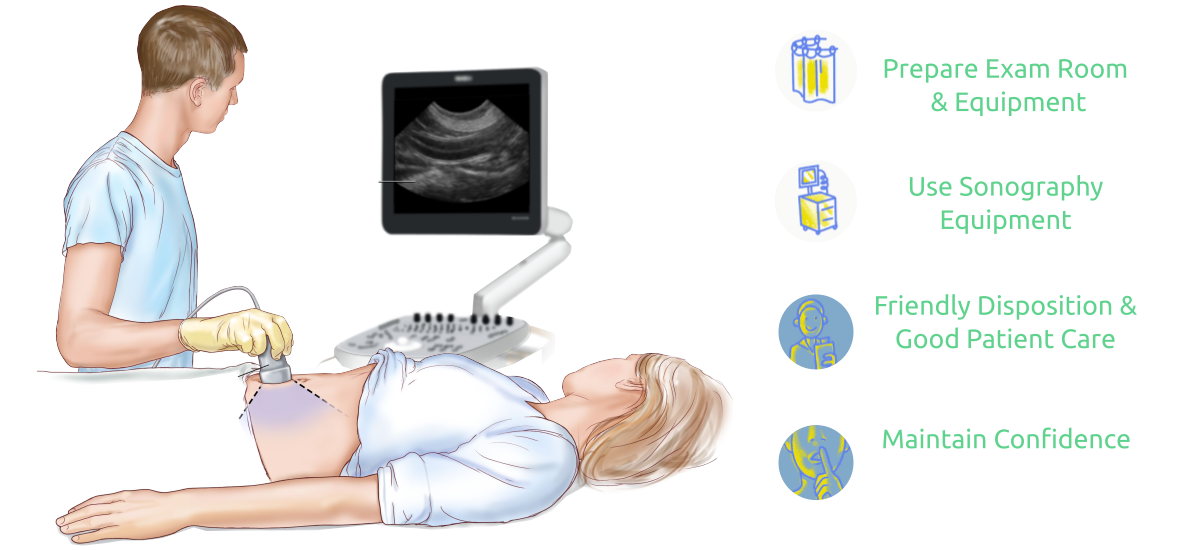
\includegraphics[width=1.0\textwidth]{./../figures/sonographer/versions/drawing-v02.png}
%        %\caption{}
%      \end{figure}
%\end{frame}
%}



%%%%%%%%%%%%%%%%%%%%%%%%%%%%%%%%%%%%%%%%%%%%
\section{Applications of Biomedical Engineering}


%%%%%%%%%%%%%%%%%%%%%%%%%%%%%%%%%%%%%%%%%%%%%%%%%%%%%%%%
{
%\paper{}
\begin{frame}{}

\BigSizeFont
\begin{center}
    How a Biomedical Engineer would help a Sonographer?
\end{center}

\end{frame}
}

%%%%%%%%%%%%%%%%%%%%%%%%%%%%%%%%%%%%%%%%%%%%%%%%%%%%%%%%
{

\paper{Fetal and Mother Numerical Models (FEMONUM) in \url{http://femonum.telecom-paristech.fr}}
%https://perso.telecom-paristech.fr/angelini/projects_research/FEMONUM/femonum_en.html
%https://perso.telecom-paristech.fr/angelini/projects_research/FEMONUM/femonum_en.html

\begin{frame}{Modelling US imaging}
      \begin{figure}
        \centering
        \includegraphics[width=1.0\textwidth]{./../figures/modelling-us-imaging/versions/drawing-v03}
        %\caption{}
      \end{figure}
\end{frame}
}




%3D slicer
%* How View Your Baby Ultrasound and Create 3D Printable Model Convert to .stl 3D Slicer for Cura
%https://www.youtube.com/watch?v=WXlwro_n3FM
%
%* View your baby ultrasound and create 3D printable model using free software
%https://www.youtube.com/watch?v=UHq0uyDvhaA
%> A couple of people has shared such data sets publicly on the Slicer forum in this topic:
%https://discourse.slicer.org/t/loading-of-ge-kretz-ultrasound-volumes-vol-file/808/40.
%For example, you can download one of the 3D baby ultrasounds in NRRD format
%(that can be loaded directly into 3D Slicer) from here: https://1drv.ms/u/s!Arm_AFxB9yqHtp93mJQfPqtsVfVeMw
%




%%%%%%%%%%%%%%%%%%%%%%%%%%%%%%%%%%%%%%%%%%%%%%%%%%%%%%%%
{
\paper{Add references}
\begin{frame}
  \frametitle{3D printing Fetuses}
  \vspace{10pt}
        \begin{figure}
        \centering
        \includegraphics[width=1.0\textwidth]{./../figures/3d-printing/why-and-how/versions/drawing-v02.png}
        %\caption{}
      \end{figure}

\end{frame}
}

%%%%%%%%%%%%%%%%%%%%%%%%%%%%%%%%%%%%%%%%%%%%%%%%%%%%%%%%%
%{
%\paper{add references}
%\begin{frame}{Simulator for Ultrasound-Guidance Interventions}
%      \begin{figure}
%        \centering
%        \includegraphics[width=0.9\textwidth]{./figures/sugi/simulator/versions/drawing-v00.png}
%        %\caption{}
%      \end{figure}
%\end{frame}
%}

%%%%%%%%%%%%%%%%%%%%%%%%%%%%%%%%%%%%%%%%%%%%%%%%%%%%%%%%%
%{
%\paper{Add references}
%\begin{frame}
%  \frametitle{3D printing Fetuses}
%  \vspace{10pt}
%  \begin{center}
%    \movie{\includegraphics[width=0.5\textwidth]{./figures/3d-printing/video-of-printing-process/versions/drawing-v01.png}}{./figures/3d-printing/video-of-printing-process/videos/apollo17.avi}
%  \end{center}
%%  \begin{itemize}
%%    \item Click on the image to play/pause the video.
%%    \item Move pointer to the bottom of the video frame for a draggable position  control.
%%  \end{itemize}
%\end{frame}
%}



%%%%%%%%%%%%%%%%%%%%%%%%%%%%%%%%%%%%%%%%%%%%%%%%%%%%%%%%
{
%\paper{}
\begin{frame}{}

\BigSizeFont
\begin{center}
    Can you identify body parts of a fetus with Ultrasound?
\end{center}
\end{frame}
}

%%%%%%%%%%%%%%%%%%%%%%%%%%%%%%%%%%%%%%%%%%%%%%%%%%%%%%%%
{

\paper{3D Slicer in \url{http://slicer.com}}

\begin{frame}{DEMO: Interactive Ultrasound Imaging }
      \begin{figure}
        \centering
        \includegraphics[width=1.0\textwidth]{./../figures/3dslicer/versions/drawing-v01.png}
        %\caption{}
      \end{figure}
\end{frame}
}




%%%%%%%%%%%%%%%%%%%%%%%%%%%%%%%%%%%%%%%%%%%%%%%%%%%%%%%%
{
\paper{Xia et al., 2017 in Scientific Reports, Wright-Gilbertson M. 2014 in PhD thesis}
    \begin{frame}{Ultrasound-guided intervention}
      \begin{figure}
        \centering
        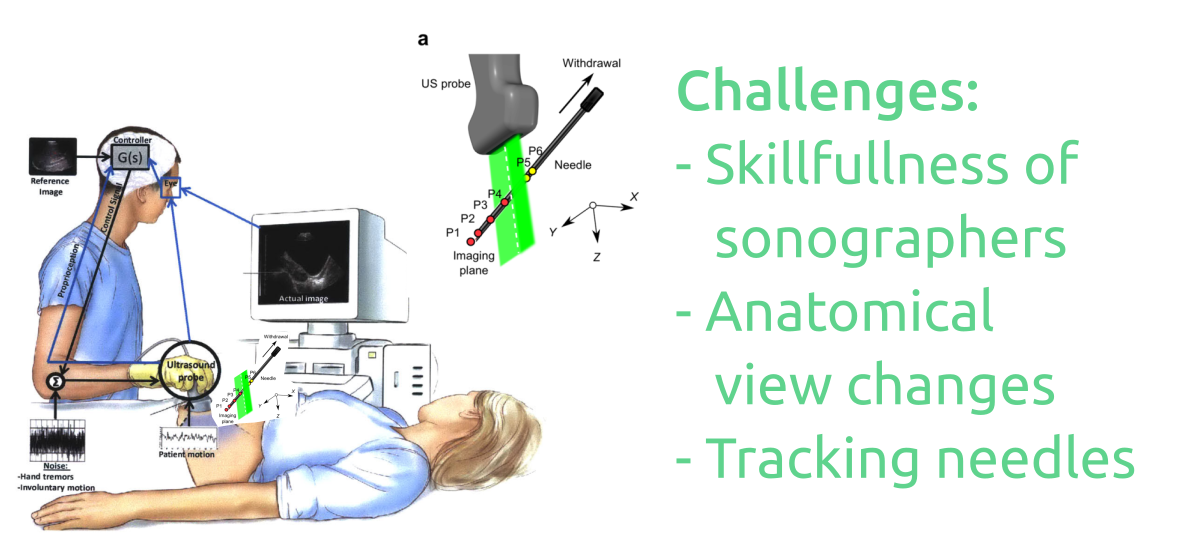
\includegraphics[width=1.0\textwidth]{./../figures/sonographer-probe-patient/versions/drawing-v03.png}
        %\caption{}
      \end{figure}
\end{frame}
}

%%%%%%%%%%%%%%%%%%%%%%%%%%%%%%%%%%%%%%%%%%%%
\section{Takeaway messages / Pop Quiz / Surprises }

%\subsection{Takeaway messages}
%\subsection{Surprises}
%\subsection{5 minutes Evaluation}


%%%%%%%%%%%%%%%%%%%%%%%%%%%%%%%%%%%%%%%%%%%%%%%%%%%%%%%%
{
%\paper{Lastname N. YEAR in journal of...}
\begin{frame}{Takeaway messages}
  \begin{figure}
  \centering
  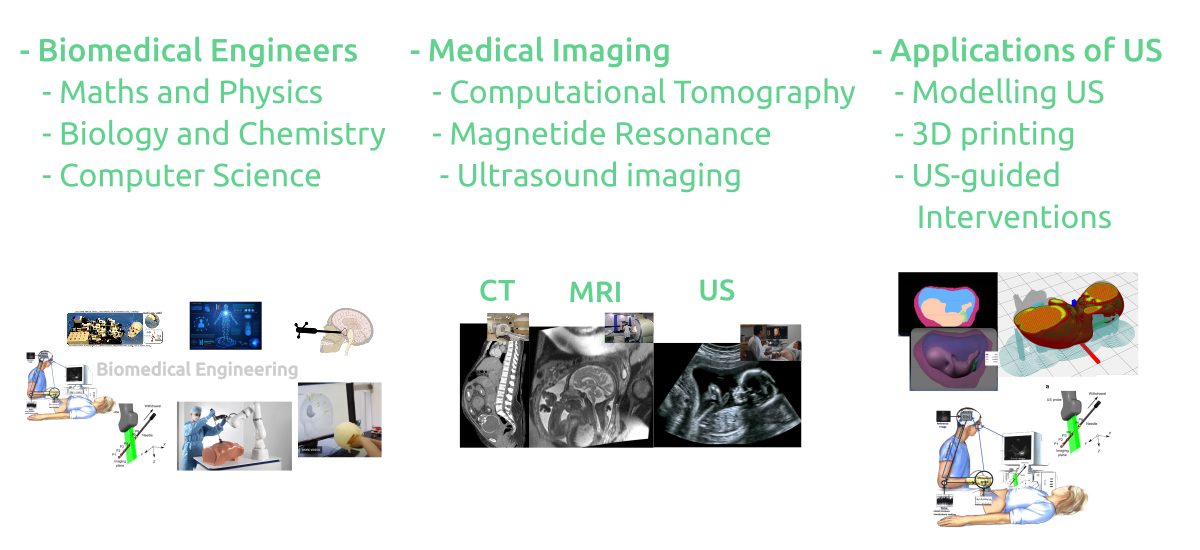
\includegraphics[width=1.0\textwidth]{./../figures/takeaways/versions/drawing-v04}
  \end{figure}

\end{frame}
}

%%%%%%%%%%%%%%%%%%%%%%%%%%%%%%%%%%%%%%%%%%%%%%%%%%%%%%%%
{
%\paper{Lastname N. YEAR in journal of...}
\begin{frame}{\faOptinMonster \faUsers ACTIVITY:  Pop Quiz and Souvenirs}
  \begin{figure}
  \centering
  \includegraphics[width=1.0\textwidth]{./../figures/popquiz-souvenirs/versions/drawing-Ss-v02}
  \end{figure}

\end{frame}
}


%%%%%%%%%%%%%%%%%%%%%%%%%%%%%%%%%%%%%%%%%%%%%%%%%%%%%%%%
{
%\paper{Lastname N. YEAR in journal of...}
\begin{frame}{\faOptinMonster \faUsers ACTIVITY:  Pop Quiz and Souvenirs}
  \begin{figure}
  \centering
  \includegraphics[width=1.0\textwidth]{./../figures/popquiz-souvenirs/versions/drawing-Qs-v01}
  \end{figure}

\end{frame}
}


%%%%%%%%%%%%%%%%%%%%%%%%%%%%%%%%%%%%%%%%%%%%%%%%%%%%%%%%
{
%\paper{Lastname N. YEAR in journal of...}
\begin{frame}{Extra Questions (EQ)}
  \begin{figure}
  \centering
  \includegraphics[width=1.0\textwidth]{./../figures/popquiz-souvenirs/versions/drawing-Qs2-v00}
  \end{figure}

\end{frame}
}



%%%%%%%%%%%%%%%%%%%%%%%%%%%%%%%%%%%%%%%%%%%%%%%%%%%%%%%%
{
%\paper{Lastname N. YEAR in journal of...}
\begin{frame}{Acknowledgements}

  \begin{figure}
  \centering
  \includegraphics[width=1.0\textwidth]{./../figures/team/versions/drawing-v05.png}
  \end{figure}

\end{frame}
}


%\begin{frame}[standout]
%  Thanks \\
%  Questions?
%\end{frame}

{
  \usebackgroundtemplate{\includegraphics[width=\paperwidth]{./../figures/background-for-titlepage/versions/drawing-v03.png}}
  \maketitle
}


\end{document}
